% Source : http://tex.stackexchange.com/questions/31518/adding-a-per-chapter-image-along-with-group-of-entries-in-toc

\documentclass{book}
	\usepackage[latin1]{inputenc}
	\usepackage[T1]{fontenc}

	\usepackage{geometry}% http://ctan.org/pkg/geometry
	\usepackage{titletoc}% http://ctan.org/pkg/titletoc
	\usepackage[export]{adjustbox}% http://ctan.org/pkg/adjustbox
	\usepackage{xparse}% http://ctan.org/pkg/xparse

	\NewDocumentCommand{\rtocstuff}{O{20pt} m O{150pt}}{% \rtocstuff[<gap>]{<content>}[<width>]
		\titlecontents{chapter}
			[0pt]% left margin indent
			{\bigskip\bfseries}% chapter ToC formatting
			{\makebox[1.5em][l]{\thecontentslabel}}% chapter label (numbered)
			{\hspace*{1.5em}}% chapter label (unnumbered)
			{%
				\titlerule*[1pc]{.}% dotted contents line
				\thecontentspage% ToC page number
				\hspace*{#1}% gap between page number & <content>
				\smash{% remove vertical height of image
					\raisebox{1.5ex}{% align with top of character
						\hspace*{#3}% space for <content>
						\llap{% left overlap
							#2% actual <content>
						}%
					}%
				}%
			}%
		\titlecontents{section}
			[0pt]% left margin indent
			{\normalfont}% section ToC formatting
			{\hspace*{1.5em}\makebox[2.3em][l]{\thecontentslabel}}% section label (numbered)
			{\hspace*{3.8em}}% section label (unnumbered)
			{%
				\titlerule*[1pc]{.}% dotted contents line
				\thecontentspage% ToC page number
				\hspace*{#1}% gap between page number & <content>
				\hspace*{#3}% gap for <content>
			}
	}
	\NewDocumentCommand{\ltocstuff}{O{150pt} m O{20pt}}{% \ltocstuff[<width>]{<content>}[<gap>]
		\titlecontents{chapter}
			[0pt]% left margin indent
			{\bigskip\bfseries}% chapter ToC formatting
			{%
				\smash{% remove vertical height of image
					\raisebox{1.5ex}{% align with top of character
						\rlap{% right overlap
							#2% actual content
						}\hspace*{#1}% space for <content>
					}%
				}%
				\hspace*{#3}% gap between <content> and ToC entries
				\makebox[1.5em][l]{\thecontentslabel}%
			}% chapter label (numbered)
			{%
				\smash{% remove vertical height of image
					\raisebox{1.5ex}{% align with top of character
						\rlap{% right overlap
							#2% actual <content>
						}\hspace*{#1}% space for <content>
					}%
				}%
				\hspace*{1.5em}%
			}% chapter label (unnumbered)
			{%
				\titlerule*[1pc]{.}% dotted contents line
				\thecontentspage% ToC page number
			}
		\titlecontents{section}
			[0pt]% left margin indent
			{\normalfont}% section ToC formatting
			{%
				\hspace*{#1}% space for <content>
				\hspace*{#3}% gap between <content> and ToC entries
				\hspace*{1.5em}\makebox[2.3em][l]{\thecontentslabel}%
			}% section label (numbered)
			{\hspace*{3.8em}}% section label (unnumbered)
			{%
				\titlerule*[1pc]{.}% dotted contents line
				\thecontentspage% ToC page number
			}
	}

	\usepackage{lipsum}% http://ctan.org/pkg/lipsum


\begin{document}

\contentsmargin{0pt}% Remove right margin in ToC
\tableofcontents

\rtocstuff{
\includegraphics[valign=T,width=75pt]{myPicture1}}
\chapter{Coordinates of points}
	\section{Rectangular coordinates} \lipsum[1]
	\section{Projections of a segment on the axes} \lipsum[2]
	\section{Distance between two points} \lipsum[3]
	\section{The mid-point of a segment} \lipsum[4]
	\section{Division of a segment in any ratio} \lipsum[5]
	\section{Oblique coordinates} \lipsum[6]

\ltocstuff{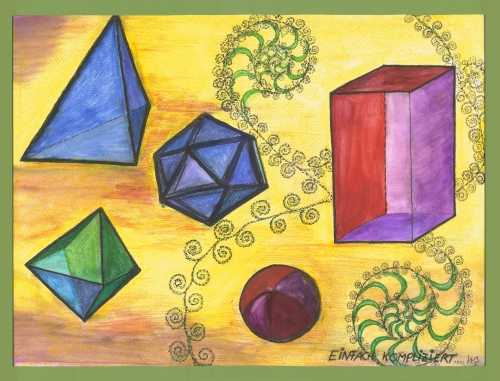
\includegraphics[valign=T,width=75pt]{myPicture2}}
\chapter{The locus of an equation}
	\section{First illustrations} \lipsum[1]
	\section{Curve plotting} \lipsum[2]
	\section{Test that a point lie on a curve} \lipsum[3]
	\section{Intercepts} \lipsum[4]
	\section{Points of intersection of two curves} \lipsum[5]
	\section{Oblique coordinates} \lipsum[6]

\rtocstuff{
\includegraphics[valign=T,width=75pt]{myPicture3}}
\chapter{The straight line}
	\section{Equation in terms of point and slope} \lipsum[1]
	\section{Line through two points} \lipsum[2]
	\section{The general equation of first degree} \lipsum[3]
	\section{Parallel and perpendicular lines} \lipsum[4]
	\section{Angle between two lines} \lipsum[5]
	\section{Distance from a point to a line} \lipsum[6]

\ltocstuff{
\includegraphics[valign=T,width=75pt]{myPicture1}}
\chapter{Coordinates of points}
	\section{Rectangular coordinates} \lipsum[1]
	\section{Projections of a segment on the axes} \lipsum[2]
	\section{Distance between two points} \lipsum[3]
	\section{The mid-point of a segment} \lipsum[4]
	\section{Division of a segment in any ratio} \lipsum[5]
	\section{Oblique coordinates} \lipsum[6]

\rtocstuff{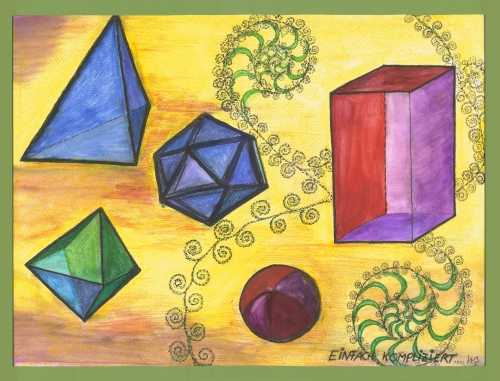
\includegraphics[valign=T,width=75pt]{myPicture2}}
\chapter{The locus of an equation}
	\section{First illustrations} \lipsum[1]
	\section{Curve plotting} \lipsum[2]
	\section{Test that a point lie on a curve} \lipsum[3]
	\section{Intercepts} \lipsum[4]
	\section{Points of intersection of two curves} \lipsum[5]
	\section{Oblique coordinates} \lipsum[6]

\ltocstuff{
\includegraphics[valign=T,width=75pt]{myPicture3}}
\chapter{The straight line}
	\section{Equation in terms of point and slope} \lipsum[1]
	\section{Line through two points} \lipsum[2]
	\section{The general equation of first degree} \lipsum[3]
	\section{Parallel and perpendicular lines} \lipsum[4]
	\section{Angle between two lines} \lipsum[5]
	\section{Distance from a point to a line} \lipsum[6]

\end{document}
